%% LyX 2.0.7.1 created this file.  For more info, see http://www.lyx.org/.
%% Do not edit unless you really know what you are doing.
\documentclass[10pt,twoside,english]{mwart}
\usepackage[LGR,T1]{fontenc}
\usepackage[latin9]{inputenc}
\usepackage{listings}
\usepackage[a4paper]{geometry}
\geometry{verbose,tmargin=3cm,bmargin=2cm,lmargin=2cm,rmargin=2cm,headheight=1cm,headsep=1cm}
\pagestyle{headings}
\setcounter{tocdepth}{2}
\usepackage{color}
\usepackage{babel}
\usepackage{array}
\usepackage{rotating}
\usepackage{float}
\usepackage{fancybox}
\usepackage{calc}
\usepackage{units}
\usepackage{textcomp}
\usepackage{multirow}
\usepackage{amsthm}
\usepackage{amsmath}
\usepackage{graphicx}
\usepackage[unicode=true,
 bookmarks=true,bookmarksnumbered=false,bookmarksopen=false,
 breaklinks=true,pdfborder={0 0 0},backref=false,colorlinks=false]
 {hyperref}
\hypersetup{pdftitle={Android Sensors Overview},
 pdfauthor={Carlo Antenucci}}

\makeatletter

%%%%%%%%%%%%%%%%%%%%%%%%%%%%%% LyX specific LaTeX commands.
\DeclareRobustCommand{\greektext}{%
  \fontencoding{LGR}\selectfont\def\encodingdefault{LGR}}
\DeclareRobustCommand{\textgreek}[1]{\leavevmode{\greektext #1}}
\DeclareFontEncoding{LGR}{}{}
\DeclareTextSymbol{\~}{LGR}{126}
%% Special footnote code from the package 'stblftnt.sty'
%% Author: Robin Fairbairns -- Last revised Dec 13 1996
\let\SF@@footnote\footnote
\def\footnote{\ifx\protect\@typeset@protect
    \expandafter\SF@@footnote
  \else
    \expandafter\SF@gobble@opt
  \fi
}
\expandafter\def\csname SF@gobble@opt \endcsname{\@ifnextchar[%]
  \SF@gobble@twobracket
  \@gobble
}
\edef\SF@gobble@opt{\noexpand\protect
  \expandafter\noexpand\csname SF@gobble@opt \endcsname}
\def\SF@gobble@twobracket[#1]#2{}
%% Because html converters don't know tabularnewline
\providecommand{\tabularnewline}{\\}

%%%%%%%%%%%%%%%%%%%%%%%%%%%%%% Textclass specific LaTeX commands.
\numberwithin{equation}{section}
\numberwithin{figure}{section}
\newenvironment{lyxcode}
{\par\begin{list}{}{
\setlength{\rightmargin}{\leftmargin}
\setlength{\listparindent}{0pt}% needed for AMS classes
\raggedright
\setlength{\itemsep}{0pt}
\setlength{\parsep}{0pt}
\normalfont\ttfamily}%
 \item[]}
{\end{list}}
  \theoremstyle{remark}
  \newtheorem*{rem*}{\protect\remarkname}
\newenvironment{lyxlist}[1]
{\begin{list}{}
{\settowidth{\labelwidth}{#1}
 \setlength{\leftmargin}{\labelwidth}
 \addtolength{\leftmargin}{\labelsep}
 \renewcommand{\makelabel}[1]{##1\hfil}}}
{\end{list}}

%%%%%%%%%%%%%%%%%%%%%%%%%%%%%% User specified LaTeX commands.
\usepackage{colortbl}
\usepackage{listings}
\definecolor{maroon}{rgb}{0.5,0,0}
\definecolor{darkgreen}{rgb}{0,0.5,0}
\definecolor{gray}{RGB}{192, 192, 192}
\lstdefinelanguage{XML}
{
  basicstyle=\ttfamily\footnotesize,
  morestring=[b]",
  moredelim=[s][\bfseries\color{darkgreen}]{<}{\ },
  moredelim=[s][\bfseries\color{darkgreen}]{</}{>},
  moredelim=[l][\bfseries\color{darkgreen}]{/>},
  moredelim=[l][\bfseries\color{darkgreen}]{>},
  morecomment=[s]{<?}{?>},
  morecomment=[s]{<!--}{-->},
  commentstyle=\color{maroon},
  stringstyle=\color{blue},
  identifierstyle=\color{magenta}
}

\@ifundefined{showcaptionsetup}{}{%
 \PassOptionsToPackage{caption=false}{subfig}}
\usepackage{subfig}
\makeatother

  \providecommand{\remarkname}{Remark}

\begin{document}

\author{ALMA MATER STUDIORUM - UNIVERSITY OF BOLOGNA}


\title{\vspace*{\fill}{\Huge{}\href{http://carloantenucci.github.io/AndroidSensorSupport/}{Android Sensors Support}}\\
{\Huge{}~}\\
{\large{}Carlo Antenucci}\\
{\small{}\href{mailto:carlo.antenucci@gmail.com}{carlo.antenucci@gmail.com}}\\
{\small{}\href{mailto:carlo.antenucci@studio.unibo.it}{carlo.antenucci@studio.unibo.it}}\\
 \vspace*{\fill}}

\maketitle
\cleardoublepage{}

\tableofcontents{}

\newpage{}
\begin{abstract}
Most Android-powered device have several built-in sensors that measure
motion, orientation and other various enviromental condition, provide
raw data with high precision and accuracy, and are useful to monitor
three-dimensional device movement and positioning or monitor changes
in the ambiental environment near a device.\\


Android platform supports three category of sensors:

\textbf{Motion~sensors}: measure acceleration and rotational forces
along three axis. This category includes \textit{accelerometer}, g\textit{ravity
sensor}, \textit{gyroscope} and \textit{rotational vector sensor}.

\textbf{Enviromental}~\textbf{sensors}: sensors included in this
category (\textit{barometer}, \textit{photometer} and \textit{thermometer})
measure various enviromental parameters such as temperature, pressure,
illumination, humidity.

P\textbf{osition~sensor}s: measure physical position of a device
using \textit{orientation sensor }and \textit{magnetometer}.\\


The access to a sensor and the raw sensor data acquisition are simplified
by using Android Sensor Framework\textbf{ }that provides several classes
and interfaces that helps developer to perform a large number of sensor-related
task.

The first part of this paper is based on the Adroid Developers sensors
documentation\cite{androidDev}: introduces the Android sensor framework
and explains how to use sensors.

In the second part is introduced a sensor and sensor data model that
realizes a new layer between Android Sensor Framework and the final
application. The model has been developed as project activity related
to the Engineering of Software System course. This layer simplifies
the sensor usage and allow a developer to ask to the sensor his data
value (Android Sensor Framework only notify a change, but developers
cannot request information to the sensor without save the last update
in a variable).

All source code and informations are available at \href{http://carloantenucci.github.io/AndroidSensorSupport/}{http://carloantenucci.github.io/AndroidSensorSupport/}\newpage{}
\end{abstract}

\section{Android Sensor Framework}


\subsection{Introduction to sensors}

The Android Sensor Framework lets access to access many type of sensors,
some of these are hardware-based (real sensors) and some are are software-based
(virtual sensors).

Hardware-based sensors are built into the device and they derive data
by directly measuring specific environmental properties, while software-based
sensors are not physical devices despite they mimic an hardware-based
sensor. This second group derive their data from one ore more of the
hardware-based sensors.

\begin{center}
\begin{table}[H]
\caption{Sensor types supported by the Android platform}


\centering{}%
\begin{tabular}{|>{\raggedright}m{0.3\columnwidth}|>{\raggedright}m{0.1\textwidth}|>{\raggedright}m{0.3\textwidth}|>{\raggedright}m{0.2\textwidth}|}
\hline 
\rowcolor{cyan}
\centering\textbf{Sensor} & \centering\textbf{Type} & \centering\textbf{Description} & \centering\textbf{Sensor fusion}\tabularnewline
\hline 
\hline 
\texttt{\footnotesize{}TYPE\_ACCELEROMETER} & {\footnotesize{}Hardware} & {\footnotesize{}Measures the acceleration force in $\nicefrac{m}{s^{2}}$
that is applied to a device on all three physical axes (x, y, and
z), including the force of gravity.} & \tabularnewline
\hline 
\texttt{\footnotesize{}TYPE\_GRAVITY} & {\footnotesize{}Software or Hardware} & {\footnotesize{}Measures the force of gravity in $\nicefrac{m}{s^{2}}$
that is applied to a device on all three physical axes (x, y, and
z).} & {\footnotesize{}If it is software uses Accelerometer to derive data}\tabularnewline
\hline 
\texttt{\footnotesize{}TYPE\_GYROSCOPE} & {\footnotesize{}Hardware} & {\footnotesize{}Measures a device's rate of rotation in $\nicefrac{rad}{s}$
that is applied to a device on all three physical axes (x, y, and
z).} & \tabularnewline
\hline 
\texttt{\footnotesize{}TYPE\_LINEAR\_ACCELERATION} & {\footnotesize{}Software} & {\footnotesize{}Measures the acceleration force in $\nicefrac{m}{s^{2}}$
that is applied to a device on all three physical axes (x, y, and
z), excluding the force of gravity.} & \begin{itemize}
\item {\footnotesize{}Acceleromter}{\footnotesize \par}
\item {\footnotesize{}Gravity sensor}\end{itemize}
\tabularnewline
\hline 
\texttt{\footnotesize{}TYPE\_ORIENTATION} & {\footnotesize{}Software} & {\footnotesize{}Measures degrees of rotation that a device makes around
all three physical axes (x, y, z). As of API level 3 you can obtain
the inclination matrix and rotation matrix for a device by using the
gravity sensor and the geomagnetic field sensor in conjunction with
the getRotationMatrix() method.} & \begin{itemize}
\item {\footnotesize{}Accelerometer}{\footnotesize \par}
\item {\footnotesize{}Geomagnetic field}\end{itemize}
\tabularnewline
\hline 
\texttt{\footnotesize{}TYPE\_ROTATION\_VECTOR} & {\footnotesize{}Software or Hardware} & {\footnotesize{}Measures the orientation of a device by providing
the three elements of the device's rotation vector.} & {\footnotesize{}If it is software uses Gyroscope to derive data}\tabularnewline
\hline 
\texttt{\footnotesize{}TYPE\_AMBIENT\_TEMPERATURE} & {\footnotesize{}Hardware} & {\footnotesize{}Measures the ambient room temperature in degrees Celsius
($\text{\textdegree C}$).} & \tabularnewline
\hline 
\texttt{\footnotesize{}TYPE\_LIGHT} & {\footnotesize{}Hardware} & {\footnotesize{}Measures the ambient illumination in lx.} & \tabularnewline
\hline 
\texttt{\footnotesize{}TYPE\_PRESSURE} & {\footnotesize{}Hardware} & {\footnotesize{}Measures the ambient air pressure in $hPa$ or $mbar$.} & \tabularnewline
\hline 
\texttt{\footnotesize{}TYPE\_RELATIVE\_HUMIDITY} & {\footnotesize{}Hardware} & {\footnotesize{}Measures the ambient humidity in percent ($\%$).} & \tabularnewline
\hline 
\texttt{\footnotesize{}TYPE\_TEMPERATURE} & {\footnotesize{}Hardware} & {\footnotesize{}Measures the temperature of the device in degree Celsius
($\text{\textdegree C}$).} & \tabularnewline
\hline 
\texttt{\footnotesize{}TYPE\_MAGNETIC\_FIELD} & {\footnotesize{}Hardware} & {\footnotesize{}Measures the ambient geomagnetic field for all three
physical axes (x, y, z) in $\mu T$.} & \tabularnewline
\hline 
\texttt{\footnotesize{}TYPE\_PROXIMITY} & {\footnotesize{}Hardware} & {\footnotesize{}Measures the proximity of an object in cm relative
to the view screen of a device. } & \tabularnewline
\hline 
\end{tabular}
\end{table}

\par\end{center}


\subsection{Android sensor framework}

Android sensor framework is part of the \texttt{android.hardware}
package. This subsystem includes the interface, named sensor Hardware
Abstraction Layer (sensor HAL), between the hardware driver and the
other framework classes and interfaces which allows developers to
\begin{itemize}
\item Indentify sensors and sensor capabilities\\
useful for application with features that needs a specific sensor
type or capabilities (identify all sensors that are present on a device
and disable features that rely on sensors not present)
\item Monitor sensor events\\
raw sensors data acquisition. Every time a sensor detects a change
(normally every x nanoseconds, with x defined by one of \texttt{SENSOR\_DELAY\_{*}}
value) in the parameter that is measuring, notify this change using
a sensor event that provides four different informations:

\begin{itemize}
\item Name of the sensor that triggered the event
\item Timestamp of the event in nanoseconds%
\footnote{An Android Project Member says: ``{[}...{]}The timestamps are not
defined as being the Unix time; they're just \textquotedbl{}a time\textquotedbl{}
that's only valid for a given sensor. {[}...{]}''\cite{TimeStamp}%
}
\item Accuracy of the event
\item Raw data that triggered the event
\end{itemize}
\end{itemize}
This tasks can be performed using the sensor-related APIs introduced
by classes and interfaces included in Android sensor framework:
\begin{description}
\item [{\texttt{\textcolor{black}{SensorManager}}}] This class creates
an instance of the sensor service and provides methods to access and
listens sensors, register and un register sensor listeners, acquire
device orientation informations and also defines several sensors constants
useful to report sensor accuracy, set data acquisition rates, and
calibrate sensors.
\item [{\texttt{\textcolor{black}{Sensor}}}] \textcolor{black}{This class
is useful to create an instance of a specific sensor and provides
various methods that determine sensor's capabilities.}
\item [{\texttt{\textcolor{black}{SensorEvent}}}] \textcolor{black}{Android
uses this class to create a sensor event object which provides sensor
event's informations such as raw sensor data, sensor type that generated
the event, event accuracy and time stamp.}
\item [{\texttt{\textcolor{black}{SensorEventListener}}}] This interface
is useful to create two callback methods that receive notification
(a sensor event) when sensor values or sensor accuracy change.
\end{description}

\subsection{Sensor availability}

Sensors availability is different within devices and is different
too among Android versions because the Android sensors have been introduced
in different platmorm releases.

Many sensors have been introduced by Android 1.5 Cupcake (API Level
3), but some were not implemented and not available until Android
2.3 Gingerbread (API Level 9) that introduces too new sensors. Other
sensors were introduced by Android 4.0 Ice Cream Sandwich (API Level
14) that also deprecates two sensors, replaced by newer and better
sensors.

The following table summarize the availability of each sensor in each
Android release.

\begin{center}
\begin{minipage}[t]{1\columnwidth}%
\begin{table}[H]
\caption{Sensor types supported by the Android platform}


\centering{}%
\begin{tabular}{|>{\raggedright}m{0.3\columnwidth}|>{\raggedright}m{0.14\textwidth}|>{\raggedright}m{0.14\textwidth}|>{\raggedright}m{0.14\textwidth}|>{\raggedright}m{0.14\textwidth}|}
\hline 
\rowcolor{cyan}
\centering\textbf{Sensor} & \centering\textbf{Android 4 }

\textbf{Ice Cream Sandwich}

(API Level 14) & \centering\textbf{Android 2.3}

\textbf{Gingerbread}

(API Level 9) & \centering\textbf{Android 2.2 }

\textbf{Froyo}

(API Level 8) & \centering\textbf{Android 1.5}

\textbf{Cupcake}

(API Level 3)\tabularnewline
\hline 
\hline 
\texttt{\footnotesize{}TYPE\_ACCELEROMETER} & YES & YES & YES & YES\tabularnewline
\hline 
\texttt{\footnotesize{}TYPE\_GRAVITY} & YES & YES & n/a & n/a\tabularnewline
\hline 
\texttt{\footnotesize{}TYPE\_GYROSCOPE} & YES & YES & n/a%
\footnote{Added in Android 1.5 (API Level 3), but not available untin Android
2.3 (API Level 9).%
} & n/a\textsuperscript{a}\tabularnewline
\hline 
\texttt{\footnotesize{}TYPE\_LINEAR\_ACCELERATION} & YES & YES & n/a & n/a\tabularnewline
\hline 
\texttt{\footnotesize{}TYPE\_ORIENTATION} & YES%
\footnote{Sensor available but deprecated%
} & YES\textsuperscript{b} & YES\textsuperscript{b} & YES\tabularnewline
\hline 
\texttt{\footnotesize{}TYPE\_ROTATION\_VECTOR} & YES & YES & n/a & n/a\tabularnewline
\hline 
\texttt{\footnotesize{}TYPE\_AMBIENT\_TEMPERATURE} & YES & n/a & n/a & n/a\tabularnewline
\hline 
\texttt{\footnotesize{}TYPE\_LIGHT} & YES & YES & YES & YES\tabularnewline
\hline 
\texttt{\footnotesize{}TYPE\_PRESSURE} & YES & YES & n/a\textsuperscript{a} & n/a\textsuperscript{a}\tabularnewline
\hline 
\texttt{\footnotesize{}TYPE\_RELATIVE\_HUMIDITY} & YES & n/a & n/a & n/a\tabularnewline
\hline 
\texttt{\footnotesize{}TYPE\_TEMPERATURE} & YES\textsuperscript{b} & YES & YES & YES\tabularnewline
\hline 
\texttt{\footnotesize{}TYPE\_MAGNETIC\_FIELD} & YES & YES & YES & YES\tabularnewline
\hline 
\texttt{\footnotesize{}TYPE\_PROXIMITY} & YES & YES & YES & YES\tabularnewline
\hline 
\end{tabular}
\end{table}
%
\end{minipage}\clearpage{}
\par\end{center}


\subsection{Sensor coordinate system}

\textcolor{black}{Generally the sensor framework uses a standard 3-axis
coordinate system to express data values.}

\textcolor{black}{X, Y and Z values are represented respectively by
}\texttt{\textcolor{black}{values{[}0{]}}}\textcolor{black}{, }\texttt{\textcolor{black}{values{[}1{]}}}\textcolor{black}{{}
and }\texttt{\textcolor{black}{values{[}2{]}}}\textcolor{black}{{} of
}\texttt{\textcolor{black}{\small{}SensorEvent}}\textcolor{black}{{}
object. Some sensors, such as proximity sensor, light sensor, pressure
sensor and temperature sensor, provides single values represented
by the only }\texttt{\textcolor{black}{values{[}0{]}}}\textcolor{black}{.}

\textcolor{black}{For }\texttt{\textcolor{black}{TYPE\_ACCELEROMETER}}\textcolor{black}{,
}\texttt{\textcolor{black}{TYPE\_GRAVITY}}\textcolor{black}{, }\texttt{\textcolor{black}{TYPE\_GYROSCOPE}}\textcolor{black}{,
}\texttt{\textcolor{black}{TYPE\_LINEAR\_ACCELERATION}}\textcolor{black}{{}
and }\texttt{\textcolor{black}{TYPE\_MAGNETIC\_FIELD}}\textcolor{black}{{}
the sensors the coordinate system is defined relatively to the device's
screen when the device in held in its default orientation (portrait
for smartphones, landscape for many tablet). When the device is in
its default orientation the X axis is horizontal and points to the
right, the Y axis is vertical and points up and the Z axis points
toward the outside of the screen face.}

\textcolor{black}{The most important thing to understand is that the
axes are not swapped when the device screen orientation changes.}

\begin{center}
\begin{figure}[H]
\caption{Sensor coordinate system\cite{intelDev}}


\centering{}\subfloat[Sensor coordinate system for smartphone]{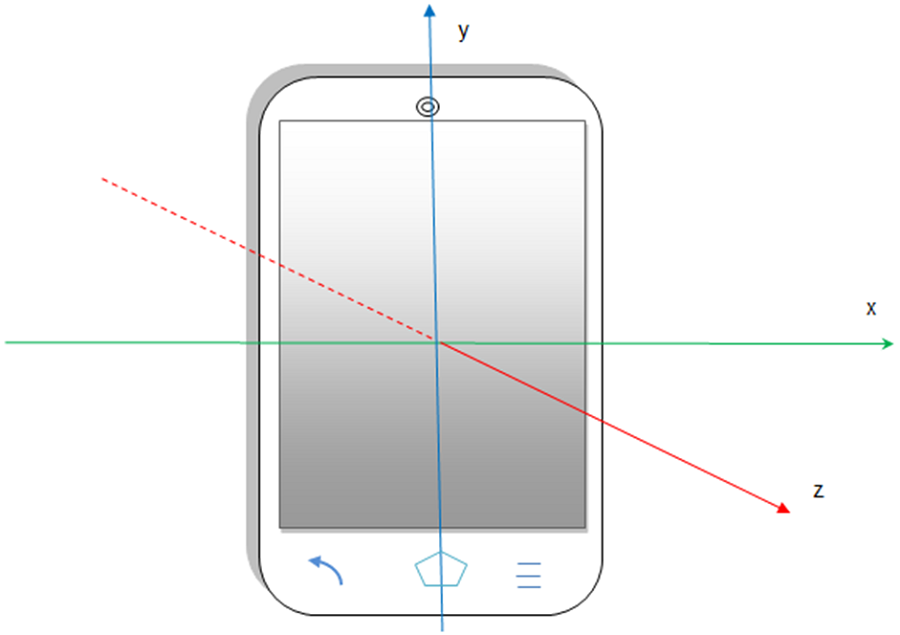
\includegraphics[width=0.3\paperwidth]{img/SensorCoordinateSystemSmartphone}}\hspace{0.05\paperwidth}\subfloat[Sensor coordinate system for tablet]{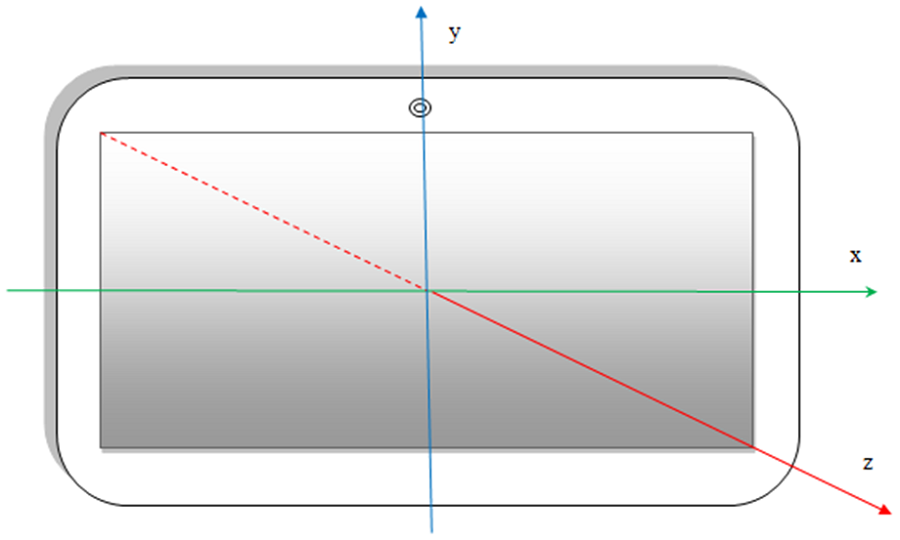
\includegraphics[width=0.3\paperwidth]{img/SensorCoordinateSystemTablet}

}
\end{figure}

\par\end{center}


\subsection{\textcolor{black}{Identifying sensors and sensor capabilities}}

\textcolor{black}{The Android sensor framework provides several methods
that make it easy determine at runtime which sensors are on a device
and the capabilities of each sensor, such as maximum range, resolution,
power requirements, minimum delay and vendor.}

\textcolor{black}{First of all, to identify the sensors on a device,
is necessary to obtain a reference to the sensor service by creating
an instance of the }\texttt{\textcolor{black}{\small{}SensorManager}}\textcolor{black}{{}
class by calling the }\texttt{\textcolor{black}{getSystemService()}}\textcolor{black}{{}
method using the }\texttt{\textcolor{black}{SENSOR\_SERVICE}}\textcolor{black}{{}
as parameter:}

\begin{center}
\textcolor{black}{}%
\ovalbox{\begin{minipage}[c]{0.77\paperwidth}%
\begin{lyxcode}
\textcolor{black}{}
\begin{lstlisting}[basicstyle={\footnotesize\sffamily},comment={[l]{//}},commentstyle={\color{darkgreen}\ttfamily},emph={int, boolean, int, float, double, List,  Sensor, SensorManager, Context},emphstyle={\color{blue}},identifierstyle={\color{black}},keywords={typeof, new, true, false, catch, function, return, null, catch, switch, var, if, in, while, do, else, case, break, int, long, this, new},keywordstyle={\color{magenta}\bfseries},language=Java,morecomment={[s]{/*}{*/}},ndkeywords={class, export, throw, implements, import, this},ndkeywordstyle={\color{darkgray}\bfseries},sensitive=false,stringstyle={\color{red}\ttfamily},tabsize=4]
private SensorManager mSensorManager;
mSensorManager = (SensorManager) getSystemService(Context.SENSOR_SERVICE);
\end{lstlisting}
\end{lyxcode}
%
\end{minipage}}
\par\end{center}

\textcolor{black}{Now, calling the}\texttt{\textbf{\textcolor{black}{{}
}}}\texttt{\textcolor{black}{getSensorList()}}\textcolor{black}{{} method
and using }\texttt{\textcolor{black}{TYPE\_ALL}}\textcolor{black}{{}
constant as parameter, }\texttt{\textcolor{black}{\small{}SensorManager}}\textcolor{black}{{}
returns the list of every sensor on the device:}

\begin{center}
\textcolor{black}{}%
\ovalbox{\begin{minipage}[c]{0.77\paperwidth}%
\begin{lyxcode}
\textcolor{black}{}
\begin{lstlisting}[basicstyle={\footnotesize\sffamily},comment={[l]{//}},commentstyle={\color{darkgreen}\ttfamily},emph={int, boolean, int, float, double, List,  Sensor, SensorManager, Context},emphstyle={\color{blue}},identifierstyle={\color{black}},keywords={typeof, new, true, false, catch, function, return, null, catch, switch, var, if, in, while, do, else, case, break, int, long, this, new},keywordstyle={\color{magenta}\bfseries},language=Java,morecomment={[s]{/*}{*/}},ndkeywords={class, export, throw, implements, import, this},ndkeywordstyle={\color{darkgray}\bfseries},sensitive=false,stringstyle={\color{red}\ttfamily},tabsize=4]
List<Sensor> deviceSensors = mSensorManager.getSensorList(Sensor.TYPE_ALL);
\end{lstlisting}
\end{lyxcode}
%
\end{minipage}}
\par\end{center}

\textcolor{black}{Using, instead of }\texttt{\textcolor{black}{TYPE\_ALL}}\textcolor{black}{{}
constant, another constant provided by }\texttt{\textcolor{black}{\small{}Sensor}}\textcolor{black}{{}
class such as }\texttt{\textcolor{black}{TYPE\_GYROSCOPE}}\textcolor{black}{,
}\texttt{\textcolor{black}{TYPE\_LINEAR\_ACCELERATION}}\textcolor{black}{,
}\texttt{\textcolor{black}{TYPE\_GRAVITY}}\textcolor{black}{{} etc.
}\texttt{\textcolor{black}{\small{}SensorManager}}\textcolor{black}{{}
class returns a lists all sensors of the given type.}

\textcolor{black}{Is also possible determine if a specific type of
sensor exists on a device by using the }\texttt{\textcolor{black}{getDefaultSensor()}}\textcolor{black}{{}
method with the sensor type constant as parameter. If a device has
more then one sensor for the given type, one of its must be designed
as the default sensor and if the default sensor does not exist, the
method returns null (which means that the device does not have thay
type of sensor). The following code checks if there is an accelerometer
on the device:}

\begin{center}
\ovalbox{\begin{minipage}[c]{0.77\paperwidth}%
\begin{lyxcode}
\begin{lstlisting}[basicstyle={\footnotesize\sffamily},comment={[l]{//}},commentstyle={\color{darkgreen}\ttfamily},emph={int, boolean, int, float, double, Sensor, SensorManager, Context},emphstyle={\color{blue}},identifierstyle={\color{black}},keywords={typeof, new, true, false, catch, function, return, null, catch, switch, var, if, in, while, do, else, case, break, int, long, this, new},keywordstyle={\color{magenta}\bfseries},language=Java,morecomment={[s]{/*}{*/}},ndkeywords={class, export, throw, implements, import, this},ndkeywordstyle={\color{darkgray}\bfseries},sensitive=false,stringstyle={\color{red}\ttfamily},tabsize=4]
private SensorManager mSensorManager;
...
mSensorManager = (SensorManager) getSystemService(Context.SENSOR_SERVICE);
if ( mSensorManager.getDefaultSensor(Sensor.TYPE_ACCELEROMETER) != null ) {
	// Success! There's an accelerometer.
}
else{
	// Failure! No accelerometer.
}
\end{lstlisting}
\end{lyxcode}
%
\end{minipage}}
\par\end{center}

\begin{center}

\par\end{center}

In addition to listing the sensors on a device, in possible, using
public methods of Sensor class, determine capabilities and attributes
of each sensor. This is useful if an application can have different
behavior depending on sensors, or sensor capabilities, available on
a device. With this methods is possible to obtain sensor's resolution
and maximum range of measurement (using \texttt{getResolution()} and
\texttt{getMaximumRange()}) or sensor's power requirement with \texttt{getPower()}
method; other two methods particularly useful to optimize an application
for different manufacturers' sensors or different sensors' version
are\texttt{ getVendor()} -for the manufacturer- and \texttt{getVersion()}
-to obtain sensor's version-.

The following sample code shows how to use \texttt{getVendor()} and
\texttt{getVersion()} methods to optimize an application using gravity
sensor if its vendor is \textsl{Google Inc.} and its version is \textsl{3},
if that particular sensor is not present on device the application
try to use the accelerometer:

Another useful methods is the \texttt{getMinDelay()} which returns
the minimum time interval (in microseconds) between two data sensed
by a sensor. Any sensor that returns a \textit{non-zero} value is
a streaming sensor -this type of sensors sense data at regular intervals
and were introduced by Android 2.3 Gingerbread (API Level 9)- while
if a sensor returns zero, it means that the sensor is not streaming
sensor, and it reports data only when there is a chenge in the paremeter
it is sensing. This method is useful because using it in possible
to determine the maximum rate at which a sensor can acquire data.

\newpage{}


\paragraph{Sensors identification code%
\footnote{This app is available on github in AboutSensors project%
}}

The following code realize an Android application that lists all sensors
in a device and its own properties. Some methods were not introduced
until API Level 9, so it works on Android 2.3 (Gingerbread) or latest.

The layout file (\texttt{\textcolor{black}{res/layout/activity\_about\_sensors.xml}})
defines the Android widgets used, their ID and their properties (position,
dimensions, alignment, etc.). In this application is needed a \texttt{\textcolor{black}{Spinner}}
to select which is the sensor to be inspected and a \texttt{\textcolor{black}{TableLayout}}
that contains a row for each property and every row contains two \texttt{\textcolor{black}{TextView}}
(a label and a value field).\\
\\
{\scriptsize{}\lstinputlisting[caption={activity\_about\_sensors.xml},language=XML]{/Users/carloantenucci/application_design/antenucci.AboutSensors/res/layout/activity_about_sensors.xml}}{\scriptsize \par}

~

The activity code is really simple: when Android system creates the
activity (\texttt{onCreate()} method), the first thing to do is the
initialization of resources. The \texttt{initializeResources()} method
assigns to each field its resource referenced in layout file, creates
the \texttt{Spinner}'s \texttt{ArrayAdapter} with sensors' names and
call the \texttt{addSpinnerListener()} method that assigns to the
\texttt{Spinner} a new \texttt{onItemSelectedListener} that changes
the shown values with the sensor selected values.\\
{\scriptsize{}\lstinputlisting[caption={AboutSensors.java},comment={[l]{//}},commentstyle={\color{darkgreen}\ttfamily},emph={int, boolean, int, float, double},emphstyle={\color{blue}},identifierstyle={\color{black}},keywords={typeof, new, true, false, catch, function, return, null, catch, switch, var, if, in, while, do, else, case, break, int, long, this, new},keywordstyle={\color{magenta}\bfseries},language={Java},language=Java,morecomment={[s]{/*}{*/}},ndkeywords={class, export, @Override},ndkeywordstyle={\color{gray}\bfseries},sensitive=false,stringstyle={\color{red}\ttfamily}]{/Users/carloantenucci/application_design/antenucci.AboutSensors/src/it/unibo/android/aboutSensors/AboutSensors.java}}{\scriptsize \par}


\subsection{Monitoring sensor events}

SensorEventListener interface introduces two callback methods which
must be implemented to monitor raw sensor data. This methods are \texttt{onAccuracyChanged()}
and \texttt{onSensorChanged()}.

This two methods are invoked by Android system, the first whenever
the sensor's accuracy changes (this method provides the reference
to the \texttt{Sensor} object that changed and its new accuracy, whose
state is represented by one of four constants defined in \texttt{SensorManager}
class:
\begin{itemize}
\item \texttt{SENSOR\_STATUS\_ACCURACY\_LOW}
\item \texttt{SENSOR\_STATUS\_ACCURACY\_MEDIUM}
\item \texttt{SENSOR\_STATUS\_ACCURACY\_HIGH}
\item \texttt{SENSOR\_STATUS\_ACCURACY\_UNRELIABLE}
\end{itemize}
The \texttt{onSensorChanged()} method, insted, is invoked by system
when a sensor reports a new value. This method provides a new \texttt{SensorEvent}
object that contains informations about the new sensor data (the new
data recorded by the sensor, its accuracy, the sensor which generates
the new data and the relative timestamp).


\paragraph{Sensor events code%
\footnote{This app is available on github in the project AboutSensorEvents%
}}

The following code is based on AboutSensors project. In this application
is shown, with the previous informations, the raw sensor data, received
by the selected sensor.

In layout file (\texttt{\textcolor{black}{res/layout/activity\_about\_sensor\_events.xml}})
above the sensor informations table is defined a new table that contains
3 rows with 3 labels and 3 \texttt{TextView}, one for each axes value
(X, Y and Z). The following code shown only the difference between
the previous and the new layout. 

\clearpage{}

This part of code begins after the \lstinline[basicstyle={\small\ttfamily},language=XML]!</TableLayout>!
tag.

{\scriptsize{}\lstinputlisting[caption={activity\_about\_sensor\_events.xml},firstline=142,language=XML]{/Users/carloantenucci/application_design/antenucci.AboutSensorEvents/res/layout/activity_about_sensor_events.xml}}\newpage{}The
activity, like the \texttt{AboutSensor} application, changes sensors
information when a new sensor is selected from \texttt{Spinner} and
shows, in addition to sensor informations, the sensor row data updated
by the sensor event listener, in fact, the \texttt{SpinnerListener},
by \texttt{onItemSelected} method, changes the \texttt{SensorEventsListener}
calling the \texttt{updateSensorListener} method, which removes old
listener from previous selected sensor and attaches to the new selected
sensor a new listener. This method is called too when the application
is resumed (\texttt{onResume()} method), and, when the application
is paused (\texttt{onPause()} method) the sensor listener is detached
from sensor.

The \texttt{SensorEventsListener} class extends \texttt{SensorEventListener}
interface the defines
\begin{itemize}
\item \texttt{onSensorChanged} method that updates the sensor data's text
views
\item \texttt{onAccuracyChanged} that, in this case, does nothing
\end{itemize}
~

{\scriptsize{}\lstinputlisting[caption={AboutSensorEvents.java},comment={[l]{//}},commentstyle={\color{darkgreen}\ttfamily},emph={int, boolean, int, float, double},emphstyle={\color{blue}},identifierstyle={\color{black}},keywords={typeof, new, true, false, catch, function, return, null, catch, switch, var, if, in, while, do, else, case, break, int, long, this, new},keywordstyle={\color{magenta}\bfseries},language={Java},morecomment={[s]{/*}{*/}},ndkeywords={class, export, @Override},ndkeywordstyle={\color{gray}\bfseries},sensitive=false,stringstyle={\color{red}\ttfamily}]{/Users/carloantenucci/application_design/antenucci.AboutSensorEvents/src/it/unibo/android/aboutSensorEvents/AboutSensorEvents.java}}{\scriptsize \par}


\subsection{Best practices for accessing and using sensors}

In this section are discussed the guidelines to design an optimized
sensor implementation. 

These guidelines are recommended best practices for anyone who is
using the sensor framework to access sensors and acquire sensor data.


\subsubsection*{Verify sensors' availability}

Android platform does not require to the manufacturer that a device
includes particular sensors, then, before using a specific sensor
it is necessary to check if this sensor exists. 

Assume the existence of a sensor simply because is frequently used
is a bad practice.


\subsubsection*{Unregister sensor listeners}

If a sensor listener is registered and its activity is paused, the
sensor will continue to acquire data and use battery resources unless
the listener is unregisterd. The bettter way to optimize resources
usage is to unregister the listener each time the application is paused,
or the sensor is no longer needed, and then register it again when
the app is resumed. This is possible using two methods provided by
the \texttt{Activity} class:
\begin{description}
\item [{\texttt{onPause()}}] called when the application is going down
(or lost the screen)
\item [{\texttt{onResume()}}] invoked when the application comes back to
the screen
\end{description}
The following code is an example that show how to use this two methods
in an \texttt{Activity} that implements \texttt{SensorEventListener}
interface:

\begin{center}
\textcolor{black}{}%
\ovalbox{\begin{minipage}[c]{0.77\paperwidth}%
\begin{lyxcode}
\textcolor{black}{}
\begin{lstlisting}[basicstyle={\footnotesize\sffamily},comment={[l]{//}},commentstyle={\color{darkgreen}\ttfamily},emph={int, boolean, int, float, double, List,  Sensor, SensorManager, Context, Bundle, ArrayList, Activity, View, AdapterView, OnItemSelectedListener, ArrayAdapter, Spinner, TextView},emphstyle={\color{blue}},identifierstyle={\color{black}},keywords={typeof, new, true, false, catch, function, return, null, catch, switch, var, if, in, while, do, else, case, break, int, long, this, new},keywordstyle={\color{magenta}\bfseries},language=Java,morecomment={[s]{/*}{*/}},ndkeywords={class, export, @Override},ndkeywordstyle={\color{gray}\bfseries},sensitive=false,stringstyle={\color{red}\ttfamily},tabsize=4]
private SensorManager mSensorManager;
private Sensor mSensor
  ... 

@Override protected void onPause() {
  super.onPause();
  mSensorManager.unregisterListener(this, mSensor);
}

@Override protected void onResume() {
  super.onResume();
  mSensorManager.registerListener(this, mSensor, SensorManager.SENSOR_DELAY_NORMAL);
}
\end{lstlisting}
\end{lyxcode}
%
\end{minipage}}
\par\end{center}


\subsubsection*{Don't test your code on the emulator}

The Android emulator cannot emulate sensors, thus, currently, is not
possible to test the sensor code on Android Virtual Devices. The best
way to run a test on sensor code is by using a physical device. There
are, however, sensor simulators that can be used to simulate sensor
output.


\subsubsection*{Don't block the\texttt{ onSensorChanged() }method}

Android system may call the \texttt{onSensorChanged(SensorEvent)}
method quite often because sensor data can changes at high rate, hence
is recommended, as the best practice, do as little is possible into
\texttt{onSensorChanged(SensorEvent)} so as not to block his execution.

If an application requires any data filtering or reduction of sensor
data, it would be better perform that work outside of the \texttt{onSensorChanged(SensorEvent)}
method.
\begin{rem*}
If the \texttt{onSensorChange(SensorEvent)} contains a loop the application
is stopped by the system.
\end{rem*}

\subsubsection*{Avoid using deprecated methods or sensor types}

Several methods and constants, such as \texttt{TYPE\_ORIENTATION}
or \texttt{TYPE\_TEMPERATURE}, have been deprecated, the first has
been replaced by \texttt{getOrientation()} method and the second,
in devices that are running Android 4 Ice Cream Sandwich, by \texttt{TYPE\_AMBIENT\_TEMPERATURE}
constant.


\subsubsection*{Choose sensor delay carefully}

The \texttt{registerListener()} method requires, in addiction to the
listener and the sensor, the minimum delay between two notifications.
The choise of the delivery rate must be suitable for the application
or use-case: sensors can provide data at very high rates and allowing
the system to send extra data which is not needed wastes system resources
and uses battery power. Like the accuracy, Android provides, in \texttt{SensorManager}
class, four differents constants that defines four different delivery
rate:
\begin{description}
\item [{\texttt{SENSOR\_DELAY\_NORMAL}}] delivery rate of 200000\textgreek{m}s 
\item [{\texttt{SENSOR\_DELAY\_UI}}] delivery rate of 60000\textgreek{m}s 
\item [{\texttt{SENSOR\_DELAY\_GAME}}] delivery rate of 20000\textgreek{m}s
\item [{\texttt{SENSOR\_DELAY\_FASTEST}}] delivery rate of 0\textgreek{m}s
(enable the real delay time of the sensor, obtained by \texttt{getMinDelay()}
method)
\end{description}

\subsection{How Android Sensor Framework works}

As mentioned, to access sensor information, developer must register
one (or more) listener to a sensor through the sensor manager, after
that Android System, according with the delay selected, calls the
call-back method (\texttt{onSensorChanged()}) passing a \texttt{SensorEvent}
object, that contains all informations, as parameter. This interaciont
can be seen like a sort of observer pattern in which the sensor represent
the observable object; when it changes its state the Android System
notifies this change to the observers (each class that implements
\texttt{SensorEventListener}) registered to the sensor through the
\texttt{SensorManager} register method.

The following image tries to represent this interaction.

\begin{center}
\begin{figure}[H]
\caption{How Android Sensor Framework works}


\centering{}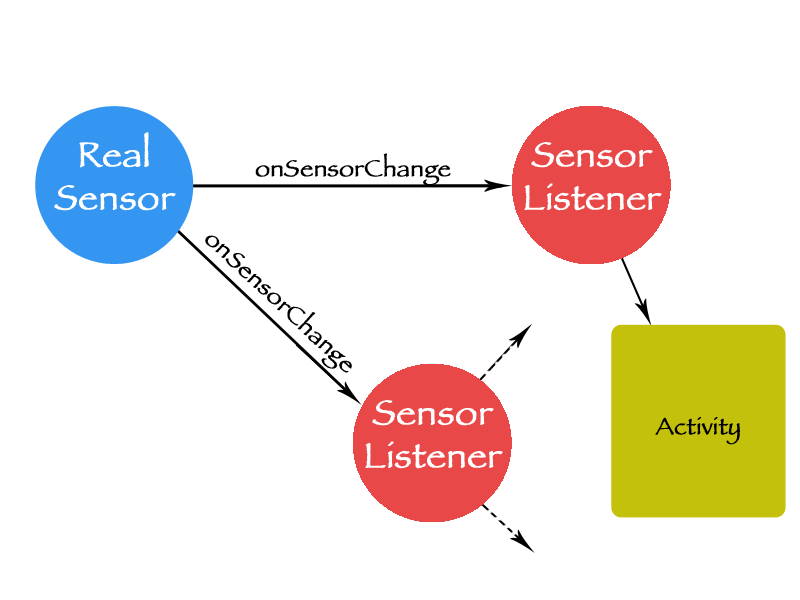
\includegraphics[width=0.4\paperwidth]{img/AndroidSensorFramework}
\end{figure}

\par\end{center}

\clearpage{}


\section{\texttt{AndroidSensorSupport}}

\texttt{AndroidSensorSupport} models Android sensors and extends the
Android Sensor Framework and simplifies the interaction with Android
sensors: each \texttt{AndroidSensor}, defined in this layer contains
a specific \texttt{AndroidSensorData} that contains all informations
relative to the last sensor update and it can be always requested
with a get method and not only when the data changes. For example,
using this layer, we can request the accelerometer data when the magnetic
field changes or vice-versa.

All \texttt{AndroidSensors} defined are, at the same time observer
(of the phisic sensor because implements \texttt{SensorEventListener})
and observable: the developer can attach to the \texttt{AndroidSensor}
a listener that does something when the data changes. The only operation
that the \texttt{AndroidSensor} does when the system calls \texttt{onSensorChanged}
is to update his sensor data and notifies this change to all his observers.

Another advantage is the \texttt{SensorFactory} that the developer
must use to obtain an \texttt{AndroidSensor}: passing to the factory
the \texttt{SensorManager} instance, the sensor type and the delay
(one of delays defined in \texttt{SensorManager} class) and it returns
an instance of \texttt{AndroidSensor} of the specific type requsted.

Last, but not least, \texttt{AndroidSensorData} contains methods to
convert it-self in strings: there are two possible representations:
\texttt{JSON} representation and Prolog-like representation that have
a functor for the data type and contains other functors for each data
(values, accuracy, timestamp, ...). Is defined also an utility class
that recostruct an \texttt{AndroidSensorData} from \texttt{JSON} string.

In the following sub-sections is analyzed the project and described
how to use this layer with a final example.


\subsection{How \texttt{AndroidSensorSupport} works}

\texttt{AndroidSensorSupport} provides a new layer between the application
and the Android Sensor Framework: now developers can insert the business
logic tha needs sensors informations directly into an observer which
is connected to the real sensor through the \texttt{AndroidSensor}
class (which implements the \texttt{SensorEventListener} and extends
the \texttt{Observable} class.

The following figure shows how the \texttt{AndroidSensorSupport} works:

\begin{center}
\begin{figure}[H]
\caption{How Android Sensor Support works}


\centering{}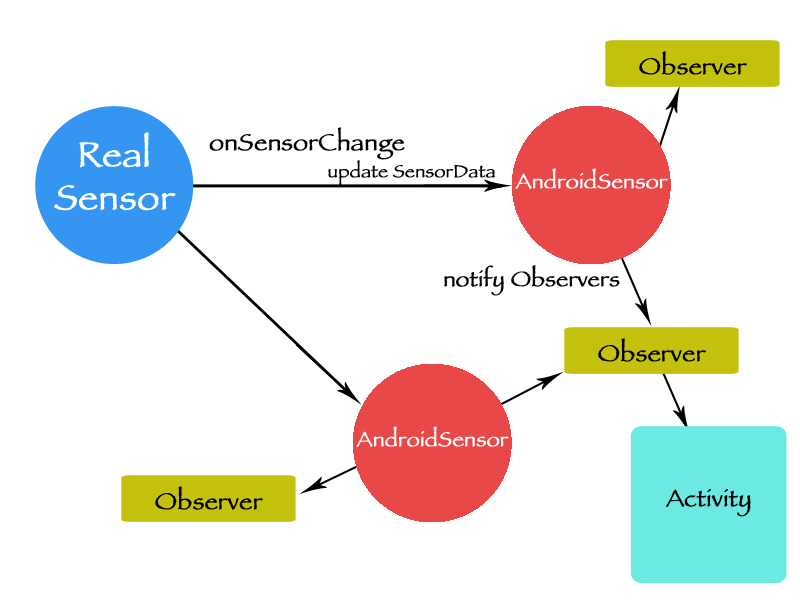
\includegraphics[width=0.4\paperwidth]{img/AndroidSensorSupport}
\end{figure}

\par\end{center}


\subsection{\texttt{AndroidSensorData} package}

The \texttt{it.unibo.android.sensorData} package contains all interfaces
and implementations that realizes the \texttt{SensorData} model. Each
sensor has a particular instance of \texttt{AndroidSensorData} that
extends the superclass as shown in the image below:

\begin{center}
\begin{figure}[H]
\caption{\texttt{SensorData} class diagram}


\centering{}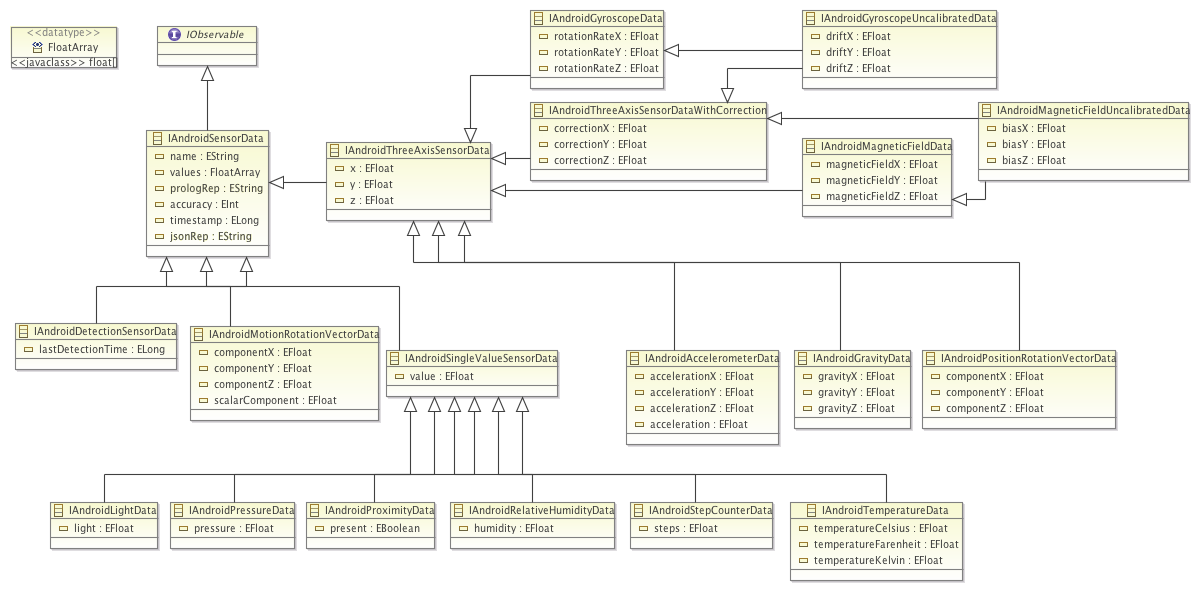
\includegraphics[width=0.9\paperwidth]{img/sensorDataUML}
\end{figure}

\par\end{center}


\subsubsection{\texttt{AndroidSensorData}}

This class provides the standard methods and variables of each subclass.
It only implements the \texttt{IObserver} interface defined in the
\texttt{uniboInterfaces.jar} library and extends the \texttt{Observable}
java class.

The following codes shows the \texttt{AndroidSensorData} interface:\\
{\scriptsize{}\lstinputlisting[caption={IAndroidSensorData.java},comment={[l]{//}},commentstyle={\color{darkgreen}\ttfamily},emph={int, boolean, int, float, double},emphstyle={\color{blue}},identifierstyle={\color{black}},keywords={typeof, new, true, false, catch, function, return, null, catch, switch, var, if, in, while, do, else, case, break, int, long, this, new},keywordstyle={\color{magenta}\bfseries},language={Java},morecomment={[s]{/*}{*/}},ndkeywords={class, export, @Override},ndkeywordstyle={\color{gray}\bfseries},sensitive=false,stringstyle={\color{red}\ttfamily}]{/Users/carloantenucci/application_design/it.unibo.android.sensorSupport/sensorData/it/unibo/android/sensorData/interfaces/IAndroidSensorData.java}}{\scriptsize \par}

This methods are useful to obtain all standard informations such as
values as array of float, accuracy, timestamp, name and the two string
representations. In the following code, is shown the implementation
of a generic \texttt{AndroidSensorData}.\\


{\scriptsize{}\lstinputlisting[caption={AndroidSensorData.java},comment={[l]{//}},commentstyle={\color{darkgreen}\ttfamily},emph={int, boolean, int, float, double},emphstyle={\color{blue}},identifierstyle={\color{black}},keywords={typeof, new, true, false, catch, function, return, null, catch, switch, var, if, in, while, do, else, case, break, int, long, this, new},keywordstyle={\color{magenta}\bfseries},language={Java},morecomment={[s]{/*}{*/}},ndkeywords={class, export, @Override},ndkeywordstyle={\color{gray}\bfseries},sensitive=false,stringstyle={\color{red}\ttfamily}]{/Users/carloantenucci/application_design/it.unibo.android.sensorSupport/sensorData/it/unibo/android/sensorData/implementation/AndroidSensorData.java}}{\scriptsize \par}

Each \texttt{AndroidSensorData} extends this class and provides specific
features for his particular case.

\clearpage{}


\subsubsection{\texttt{AndroidSingleValueSensorData}}

This class adds to the \texttt{AndroidSensorData} only one method
that returns the single value measured by the sensor:\\


{\scriptsize{}\lstinputlisting[caption={IAndroidSingleValueSensorData.java},comment={[l]{//}},commentstyle={\color{darkgreen}\ttfamily},emph={int, boolean, int, float, double},emphstyle={\color{blue}},identifierstyle={\color{black}},keywords={typeof, new, true, false, catch, function, return, null, catch, switch, var, if, in, while, do, else, case, break, int, long, this, new},keywordstyle={\color{magenta}\bfseries},language={Java},morecomment={[s]{/*}{*/}},ndkeywords={class, export, @Override},ndkeywordstyle={\color{gray}\bfseries},sensitive=false,stringstyle={\color{red}\ttfamily}]{/Users/carloantenucci/application_design/it.unibo.android.sensorSupport/sensorData/it/unibo/android/sensorData/interfaces/IAndroidSingleValueSensorData.java}}{\scriptsize \par}

In the implementation is extended the constructor that saves in a
variable the measured value (\texttt{value{[}0{]}} passed as argument)
and overrides the \texttt{getPrologRep()} method:\\
{\scriptsize{}\lstinputlisting[caption={AndroidSingleValueSensorData.java},comment={[l]{//}},commentstyle={\color{darkgreen}\ttfamily},emph={int, boolean, int, float, double},emphstyle={\color{blue}},identifierstyle={\color{black}},keywords={typeof, new, true, false, catch, function, return, null, catch, switch, var, if, in, while, do, else, case, break, int, long, this, new},keywordstyle={\color{magenta}\bfseries},language={Java},morecomment={[s]{/*}{*/}},ndkeywords={class, export, @Override},ndkeywordstyle={\color{gray}\bfseries},sensitive=false,stringstyle={\color{red}\ttfamily}]{/Users/carloantenucci/application_design/it.unibo.android.sensorSupport/sensorData/it/unibo/android/sensorData/implementation/AndroidSingleValueSensorData.java}}{\scriptsize \par}

From this class are extended other subclasses that provides specific
methods that calls the super \texttt{getValue()} and in some cases
had a conversion:
\begin{description}
\item [{\texttt{IAndroidLightData}}]~

\begin{itemize}
\item \texttt{getLight()}; returns the light in lx.
\end{itemize}
\item [{\texttt{IAndroidPressureData}}]~

\begin{itemize}
\item \texttt{getPressure()}; returns the pressure in hPa or mbar.
\end{itemize}
\item [{\texttt{IAndroidProximityData}}]~

\begin{itemize}
\item \texttt{isPresent()}; this method returns a boolean: if the device
detects something returns true.
\end{itemize}
\item [{\texttt{IAndroidRelativeHumidity}}]~

\begin{itemize}
\item \texttt{getHumidity()}; returns the relative humidity in \%.
\end{itemize}
\item [{\texttt{IAndroidTemperatureData}}]~

\begin{itemize}
\item \texttt{getTemperatureCelsius()}; returns the temperature in Celsius
degrees.
\item \texttt{getTemperatureFarenheit()}; returns the temperature in Farenheit
degrees.
\item \texttt{getTemperatureKelvin()}; returns the temperature in Kelvin
degrees.
\end{itemize}
\end{description}
\clearpage{}


\subsubsection{\texttt{AndroidThreeAxisSensorData}}

This class defines the standard \texttt{SensorData} for each three
axis sensor (accelerometer, gyroscope, etc.). It adds to the \texttt{AndroidSensorData}
three methods (one for each axis' values)\\


{\scriptsize{}\lstinputlisting[caption={IAndroidThreeAxisSensorData.java},comment={[l]{//}},commentstyle={\color{darkgreen}\ttfamily},emph={int, boolean, int, float, double},emphstyle={\color{blue}},identifierstyle={\color{black}},keywords={typeof, new, true, false, catch, function, return, null, catch, switch, var, if, in, while, do, else, case, break, int, long, this, new},keywordstyle={\color{magenta}\bfseries},language={Java},morecomment={[s]{/*}{*/}},ndkeywords={class, export, @Override},ndkeywordstyle={\color{gray}\bfseries},sensitive=false,stringstyle={\color{red}\ttfamily}]{/Users/carloantenucci/application_design/it.unibo.android.sensorSupport/sensorData/it/unibo/android/sensorData/interfaces/IAndroidThreeAxisSensorData.java}}{\scriptsize \par}

Like the \texttt{AndroidSingleValueSensorData} it defines a variable
for each axis' value, extends the constructor and overrides the \texttt{getPrologRep()}
method:\\


{\scriptsize{}\lstinputlisting[caption={AndroidThreeAxisSensorData.java},comment={[l]{//}},commentstyle={\color{darkgreen}\ttfamily},emph={int, boolean, int, float, double},emphstyle={\color{blue}},identifierstyle={\color{black}},keywords={typeof, new, true, false, catch, function, return, null, catch, switch, var, if, in, while, do, else, case, break, int, long, this, new},keywordstyle={\color{magenta}\bfseries},language={Java},morecomment={[s]{/*}{*/}},ndkeywords={class, export, @Override},ndkeywordstyle={\color{gray}\bfseries},sensitive=false,stringstyle={\color{red}\ttfamily}]{/Users/carloantenucci/application_design/it.unibo.android.sensorSupport/sensorData/it/unibo/android/sensorData/implementation/AndroidThreeAxisSensorData.java}}{\scriptsize \par}

and, still other \texttt{SensorData}, each class that extends this
have specific methods:
\begin{description}
\item [{\texttt{IAndroidAccelerometerData}}]~

\begin{itemize}
\item \texttt{getAccelerationX()}; returns the acceleration value along
the X axis;
\item \texttt{getAccelerationY()}; returns the acceleration value along
the Y axis;
\item \texttt{getAccelerationZ()}; returns the acceleration value along
the Z axis;
\item \texttt{getAcceleration()}; returns the device's acceleration calculating
as $\sqrt{a_{x}^{2}+a_{y}^{2}+a_{z}^{2}}$
\end{itemize}
\item [{\texttt{IAndroidGravityData}}]~

\begin{itemize}
\item \texttt{getGravityX()}; returns the gravity value along the X axis;
\item \texttt{getGravityY()}; returns the gravity value along the Y axis;
\item \texttt{getGravityZ()}; returns the gravity value along the Z axis
\end{itemize}
\item [{\texttt{IAndroidGyroscopeData}}]~

\begin{itemize}
\item \texttt{getRotationRateX()}; returns the rotation rate value around
the X axis;
\item \texttt{getRotationRateY()}; returns the rotation rate value around
the Y axis;
\item \texttt{getRotationRateZ()}; returns the rotation rate value around
the Z axis
\end{itemize}
\item [{\texttt{IAndroidMagneticFieldData}}]~

\begin{itemize}
\item \texttt{getMagneticFieldX()}; returns the magnetic field value along
the X axis;
\item \texttt{getMagneticFieldY()}; returns the magnetic field value along
the Y axis;
\item \texttt{getMagneticFieldZ()}; returns the magnetic field value along
the Z axis
\end{itemize}
\item [{\texttt{IAndroidPositionRotationVectorData}}]~

\begin{itemize}
\item \texttt{getComponentX()}; returns the rotation component value around
the X axis;
\item \texttt{getComponentY()}; returns the rotation component value around
the Y axis;
\item \texttt{getComponentZ()}; returns the rotation component value around
the Z axis
\end{itemize}
\end{description}

\subsubsection{\texttt{AndroidThreeAxisSensorDataWithCorrection}}

This class extends the \texttt{ThreeAxisSensorData} and adds to it
other three values that represents the correction applied by the system
accordin to the sensor informations:\\
{\scriptsize{}\lstinputlisting[caption={IAndroidThreeAxisSensorDataWithCorrection.java},comment={[l]{//}},commentstyle={\color{darkgreen}\ttfamily},emph={int, boolean, int, float, double},emphstyle={\color{blue}},identifierstyle={\color{black}},keywords={typeof, new, true, false, catch, function, return, null, catch, switch, var, if, in, while, do, else, case, break, int, long, this, new},keywordstyle={\color{magenta}\bfseries},language={Java},morecomment={[s]{/*}{*/}},ndkeywords={class, export, @Override},ndkeywordstyle={\color{gray}\bfseries},sensitive=false,stringstyle={\color{red}\ttfamily}]{/Users/carloantenucci/application_design/it.unibo.android.sensorSupport/sensorData/it/unibo/android/sensorData/interfaces/IAndroidThreeAxisSensorDataWithCorrection.java}}{\scriptsize \par}

Like the other subclasses it defines a variable for each axis' correction
values, extends the constructor and overrides the \texttt{getPrologRep()}
method:\\


{\scriptsize{}\lstinputlisting[caption={AndroidThreeAxisSensorDataWithCorrection.java},comment={[l]{//}},commentstyle={\color{darkgreen}\ttfamily},emph={int, boolean, int, float, double},emphstyle={\color{blue}},identifierstyle={\color{black}},keywords={typeof, new, true, false, catch, function, return, null, catch, switch, var, if, in, while, do, else, case, break, int, long, this, new},keywordstyle={\color{magenta}\bfseries},language={Java},morecomment={[s]{/*}{*/}},ndkeywords={class, export, @Override},ndkeywordstyle={\color{gray}\bfseries},sensitive=false,stringstyle={\color{red}\ttfamily}]{/Users/carloantenucci/application_design/it.unibo.android.sensorSupport/sensorData/it/unibo/android/sensorData/implementation/AndroidThreeAxisSensorDataWithCorrection.java}}The
only two sensors that have this type of data representation are the
\texttt{GyroscopeUncalibrated} and the \texttt{MagneticFieldUncalibrated}
and their data representation extends this class but implements also
the \texttt{GyroscopeData} or \texttt{MagneticFieldData} representation.
In the following code is show the \texttt{AndroidGyroscopeUncalibratedData},
for the \texttt{AndroidMagneticFieldUncalibratedData} the implementation
is similar, the only difference is the name of get methods for correction
(the gyroscope have \texttt{getDrift} and the magnetic field have
\texttt{getBias}):

{\scriptsize{}\lstinputlisting[caption={IAndroidGyroscopeUncalibratedData.java},comment={[l]{//}},commentstyle={\color{darkgreen}\ttfamily},emph={int, boolean, int, float, double},emphstyle={\color{blue}},identifierstyle={\color{black}},keywords={typeof, new, true, false, catch, function, return, null, catch, switch, var, if, in, while, do, else, case, break, int, long, this, new},keywordstyle={\color{magenta}\bfseries},language={Java},morecomment={[s]{/*}{*/}},ndkeywords={class, export, @Override},ndkeywordstyle={\color{gray}\bfseries},sensitive=false,stringstyle={\color{red}\ttfamily}]{/Users/carloantenucci/application_design/it.unibo.android.sensorSupport/sensorData/it/unibo/android/sensorData/interfaces/motionSensors/IAndroidGyroscopeUncalibratedData.java}}{\scriptsize \par}

{\scriptsize{}\lstinputlisting[caption={AndroidGyroscopeUncalibratedData.java},comment={[l]{//}},commentstyle={\color{darkgreen}\ttfamily},emph={int, boolean, int, float, double},emphstyle={\color{blue}},identifierstyle={\color{black}},keywords={typeof, new, true, false, catch, function, return, null, catch, switch, var, if, in, while, do, else, case, break, int, long, this, new},keywordstyle={\color{magenta}\bfseries},language={Java},morecomment={[s]{/*}{*/}},ndkeywords={class, export, @Override},ndkeywordstyle={\color{gray}\bfseries},sensitive=false,stringstyle={\color{red}\ttfamily}]{/Users/carloantenucci/application_design/it.unibo.android.sensorSupport/sensorData/it/unibo/android/sensorData/implementation/motionSensors/AndroidGyroscopeUncalibratedData.java}}{\scriptsize \par}


\subsubsection{\texttt{AndroidMotionRotationVectorData}}

This class realizes the data representation for a motion rotation
vector sensor. It is different form a \texttt{PositionRotationVectorData}
because he can have 4 values: the same of position rotation vector
and a scalar component:

{\scriptsize{}\lstinputlisting[caption={IAndroidMotionVectorRotationData.java},comment={[l]{//}},commentstyle={\color{darkgreen}\ttfamily},emph={int, boolean, int, float, double},emphstyle={\color{blue}},identifierstyle={\color{black}},keywords={typeof, new, true, false, catch, function, return, null, catch, switch, var, if, in, while, do, else, case, break, int, long, this, new},keywordstyle={\color{magenta}\bfseries},language={Java},morecomment={[s]{/*}{*/}},ndkeywords={class, export, @Override},ndkeywordstyle={\color{gray}\bfseries},sensitive=false,stringstyle={\color{red}\ttfamily}]{/Users/carloantenucci/application_design/it.unibo.android.sensorSupport/sensorData/it/unibo/android/sensorData/interfaces/motionSensors/IAndroidMotionRotationVectorData.java}}{\scriptsize \par}

{\scriptsize{}\lstinputlisting[caption={AndroidMotionVectorRotationData.java},comment={[l]{//}},commentstyle={\color{darkgreen}\ttfamily},emph={int, boolean, int, float, double},emphstyle={\color{blue}},identifierstyle={\color{black}},keywords={typeof, new, true, false, catch, function, return, null, catch, switch, var, if, in, while, do, else, case, break, int, long, this, new},keywordstyle={\color{magenta}\bfseries},language={Java},morecomment={[s]{/*}{*/}},ndkeywords={class, export, @Override},ndkeywordstyle={\color{gray}\bfseries},sensitive=false,stringstyle={\color{red}\ttfamily}]{/Users/carloantenucci/application_design/it.unibo.android.sensorSupport/sensorData/it/unibo/android/sensorData/implementation/motionSensors/AndroidMotionRotationVectorData.java}}{\scriptsize \par}


\subsubsection{\texttt{AndroidDetectionSensorData}}

This kind of sensor data representation is different from the others:
it don't have any value and the only thing that it save is the real
time of the detection (when the constructor is called):\\


{\scriptsize{}\lstinputlisting[caption={IAndroidDetectionSensorData.java},comment={[l]{//}},commentstyle={\color{darkgreen}\ttfamily},emph={int, boolean, int, float, double},emphstyle={\color{blue}},identifierstyle={\color{black}},keywords={typeof, new, true, false, catch, function, return, null, catch, switch, var, if, in, while, do, else, case, break, int, long, this, new},keywordstyle={\color{magenta}\bfseries},language={Java},morecomment={[s]{/*}{*/}},ndkeywords={class, export, @Override},ndkeywordstyle={\color{gray}\bfseries},sensitive=false,stringstyle={\color{red}\ttfamily}]{/Users/carloantenucci/application_design/it.unibo.android.sensorSupport/sensorData/it/unibo/android/sensorData/interfaces/IAndroidDetectionSensorData.java}}{\scriptsize \par}

{\scriptsize{}\lstinputlisting[caption={AndroidDetectionSensorData.java},comment={[l]{//}},commentstyle={\color{darkgreen}\ttfamily},emph={int, boolean, int, float, double},emphstyle={\color{blue}},identifierstyle={\color{black}},keywords={typeof, new, true, false, catch, function, return, null, catch, switch, var, if, in, while, do, else, case, break, int, long, this, new},keywordstyle={\color{magenta}\bfseries},language={Java},morecomment={[s]{/*}{*/}},ndkeywords={class, export, @Override},ndkeywordstyle={\color{gray}\bfseries},sensitive=false,stringstyle={\color{red}\ttfamily}]{/Users/carloantenucci/application_design/it.unibo.android.sensorSupport/sensorData/it/unibo/android/sensorData/implementation/AndroidDetectionSensorData.java}}Is
needed an override of \texttt{getValues()} method because he don't
have values, so is correct that this method returns null and is also
necessary to add another constructor that have the detection time
as parameter for the \texttt{JSON} reconstruction.


\subsubsection{\texttt{AndroidSensorDataUtils}}

This is a static class that provides a reconstruction of \texttt{SensorData}
object from a \texttt{JSON} string. It only contains a static method
that obtain information using a \texttt{JSON} parser and then, according
with the name, calls the specific constructor of \texttt{SensorData}:\\
{\scriptsize{}\lstinputlisting[caption={AndroidSensorDataUtils.java},comment={[l]{//}},commentstyle={\color{darkgreen}\ttfamily},emph={int, boolean, int, float, double},emphstyle={\color{blue}},identifierstyle={\color{black}},keywords={typeof, new, true, false, catch, function, return, null, catch, switch, var, if, in, while, do, else, case, break, int, long, this, new},keywordstyle={\color{magenta}\bfseries},language={Java},morecomment={[s]{/*}{*/}},ndkeywords={class, export, @Override},ndkeywordstyle={\color{gray}\bfseries},sensitive=false,stringstyle={\color{red}\ttfamily}]{/Users/carloantenucci/application_design/it.unibo.android.sensorSupport/sensorData/it/unibo/android/sensorData/utils/AndroidSensorDataUtils.java}}{\scriptsize \par}


\subsection{\texttt{AndroidSensorSupport} package}

The \texttt{AndroidSensorSupport} package contains all classes that
describe a sensor, extending the Android's idea of sensor. As mentioned
for Android a sensor data cannot be asked to the sensor and sensors
doesn't have a variable that contains last update values. These classes
implements the Android's \texttt{SensorEventListener} interface and
also \texttt{IObserver} and \texttt{IObservable} interfaces defined
in \texttt{uniboInterfaces.jar} contained in \texttt{it.unibo.iss.libs}.
Each sensor extends the \texttt{Observable} class, so the developer
can attach observer(s) eachone can do different tasks, without interferences
with the sensor update (this is the only operation that the \texttt{onSensorChange()}
method does, followed by the update of observers).

The following image represent the diagram class of the \texttt{AndroidSensorSupport}
package:

\begin{center}
\begin{figure}[H]
\caption{SensorSupport class diagram}


\centering{}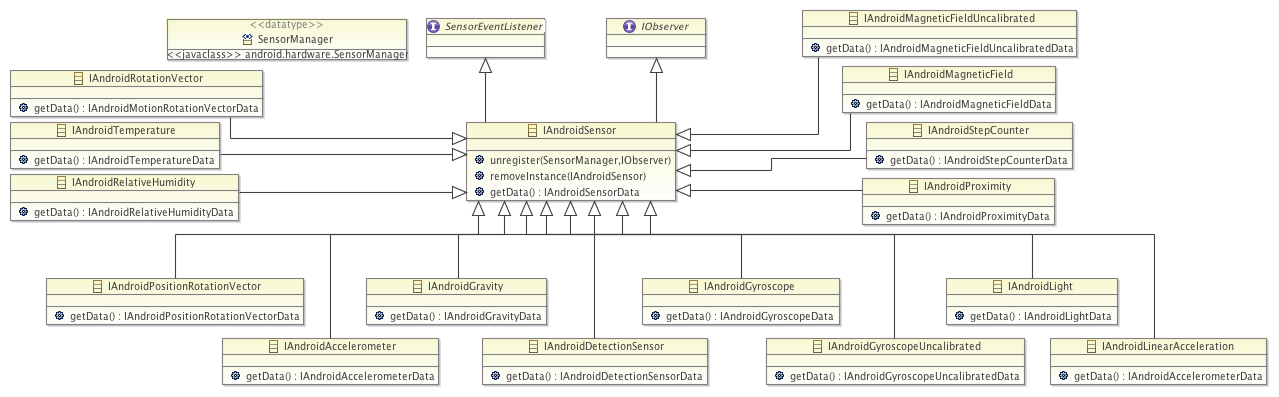
\includegraphics[width=0.9\paperwidth]{img/sensorSupport}
\end{figure}

\par\end{center}

\clearpage{}


\subsubsection{\texttt{AndroidSensor}}

\texttt{AndroidSensor} is the superclass that defines all methods
that each sensor must provide to the developer. The interface shows
only methods usefull for the developer :

{\scriptsize{}\lstinputlisting[caption={IAndroidSensor.java},comment={[l]{//}},commentstyle={\color{darkgreen}\ttfamily},emph={int, boolean, int, float, double},emphstyle={\color{blue}},identifierstyle={\color{black}},keywords={typeof, new, true, false, catch, function, return, null, catch, switch, var, if, in, while, do, else, case, break, int, long, this, new},keywordstyle={\color{magenta}\bfseries},language={Java},morecomment={[s]{/*}{*/}},ndkeywords={class, export, @Override},ndkeywordstyle={\color{gray}\bfseries},sensitive=false,stringstyle={\color{red}\ttfamily}]{/Users/carloantenucci/application_design/it.unibo.android.sensorSupport/sensorSupport/it/unibo/android/sensorSupport/interfaces/IAndroidSensor.java}}{\scriptsize \par}

{\scriptsize{}\lstinputlisting[caption={AndroidSensor.java},comment={[l]{//}},commentstyle={\color{darkgreen}\ttfamily},emph={int, boolean, int, float, double},emphstyle={\color{blue}},identifierstyle={\color{black}},keywords={typeof, new, true, false, catch, function, return, null, catch, switch, var, if, in, while, do, else, case, break, int, long, this, new},keywordstyle={\color{magenta}\bfseries},language={Java},morecomment={[s]{/*}{*/}},ndkeywords={class, export, @Override},ndkeywordstyle={\color{gray}\bfseries},sensitive=false,stringstyle={\color{red}\ttfamily}]{/Users/carloantenucci/application_design/it.unibo.android.sensorSupport/sensorSupport/it/unibo/android/sensorSupport/implementations/AndroidSensor.java}}The
interfaces describes all methods useful for the developer:
\begin{description}
\item [{\texttt{unregister()}}] removes all observers and unregister the
\texttt{AndroidSensor} from the \texttt{SensorManager}. Usefull when
the application goes \texttt{onPause()}
\item [{\texttt{getData()}}] returns the last updated \texttt{SensorData}.
In this class returns a generic \texttt{SensorData}, but in subclasses
this method is overwritten by another \texttt{getData()} that returns
the specific \texttt{SensorData}.
\end{description}
while the implementation defines also all ``background'' method: 
\begin{description}
\item [{\texttt{onSensorChanged()}}] inherited from \texttt{SensorEventListener},
that in this case only updates the \texttt{SensorData}. In subclassess
also call the update method.
\item [{\texttt{update()}}] inherited from the \texttt{Observable} class.
Set his value as changed and then send a notification to all observers
with the update data.
\item [{\texttt{addObserver()}}] inherited from the \texttt{Observable}
class. Only call the super method.
\end{description}
As mentioned, all subclasses 
\begin{itemize}
\item overrides the \texttt{onSensorChange()} method updating the specific
\texttt{SensorData} and then calls the update method passing as paramenter
the new \texttt{SensorData}.
\item overrides the \texttt{unregister()} method: deletes the instance from
the instances list and then calls the super method.
\item overwrite the \texttt{getData()} method with a specific method that
returns a specific type of \texttt{SensorData}.
\item defines a \texttt{getInstance()} method that, if exist, returns an
instance of the specific \texttt{AndroidSensor} requested, else calls
the constructor and then return this instance.
\item defines a private constructor that register the \texttt{AndroidSensor}
to the \texttt{SensorManager} and initialize a new \texttt{SensorData}
as null (until the first update is not received).
\end{itemize}
The following code shows an \texttt{AndroidAccelerometer}. In the
interface the only method introduced is the new \texttt{getData()}
that returns an \texttt{IAndroidAccelerometerData}, while in the implementation
are defined the methods described above:

{\scriptsize{}\lstinputlisting[caption={AndroidAccelerometer.java},comment={[l]{//}},commentstyle={\color{darkgreen}\ttfamily},emph={int, boolean, int, float, double},emphstyle={\color{blue}},identifierstyle={\color{black}},keywords={typeof, new, true, false, catch, function, return, null, catch, switch, var, if, in, while, do, else, case, break, int, long, this, new},keywordstyle={\color{magenta}\bfseries},language={Java},morecomment={[s]{/*}{*/}},ndkeywords={class, export, @Override},ndkeywordstyle={\color{gray}\bfseries},sensitive=false,stringstyle={\color{red}\ttfamily}]{/Users/carloantenucci/application_design/it.unibo.android.sensorSupport/sensorSupport/it/unibo/android/sensorSupport/implementations/motionSensors/AndroidAccelerometer.java}}{\scriptsize \par}

For each other sensor the implementation is the same, the only difference
is the type of \texttt{SensorData} and the type of the instances list
(obviously is the same of the \texttt{AndroidSensor}). For the \texttt{SensorData}
type is possible to reference with the following table that realizes
a match between the sensor type defined by Android, and the new \texttt{AndroidSensor}
classess with the \texttt{AndroidSensorData}:

\begin{center}
\begin{minipage}[t]{1\columnwidth}%
\begin{center}
\begin{table}[H]
\caption{Relation between Sensor Type, AndroidSensors and AndroidSensorData}


\centering{}%
\begin{tabular}{|>{\raggedright}m{0.01\columnwidth}|>{\raggedright}m{0.3\columnwidth}|>{\raggedright}m{0.3\textwidth}|>{\raggedright}m{0.35\textwidth}|}
\hline 
\rowcolor{cyan}
\centering & \texttt{\footnotesize{}\centering}\texttt{\textbf{\footnotesize{}Sensor
type}} & \texttt{\footnotesize{}\centering}\texttt{\textbf{\footnotesize{}AndroidSensor}} & \texttt{\footnotesize{}\centering}\texttt{\textbf{\footnotesize{}AndroidSensorData}}\tabularnewline
\hline 
\hline 
\multirow{5}{0.01\columnwidth}{\begin{sideways}
{\footnotesize{}Env. Sensors}
\end{sideways}} & \texttt{\footnotesize{}TYPE\_AMBIENT\_TEMPERATURE} & \texttt{\footnotesize{}AndroidTemperature} & \texttt{\footnotesize{}AndroidTemperatureData}\tabularnewline
\cline{2-4} 
 & \texttt{\footnotesize{}TYPE\_LIGHT} & \texttt{\footnotesize{}AndroidLight} & \texttt{\footnotesize{}AndroidLightData}\tabularnewline
\cline{2-4} 
 & \texttt{\footnotesize{}TYPE\_PRESSURE} & \texttt{\footnotesize{}AndroidPressure} & \texttt{\footnotesize{}AndroidPressureData}\tabularnewline
\cline{2-4} 
 & \texttt{\footnotesize{}TYPE\_RELATIVE\_HUMIDITY} & \texttt{\footnotesize{}AndroidRelativeHumidity} & \texttt{\footnotesize{}AndroidRelativeHumidityData}\tabularnewline
\cline{2-4} 
 & \texttt{\footnotesize{}TYPE\_TEMPERATURE}%
\footnote{This sensor type is replaced in Android 4.0 (API Level 14) with TYPE\_AMBIENT\_TEMPERATURE. %
} & \texttt{\footnotesize{}AndroidTemperature} & \texttt{\footnotesize{}AndroidTemperatureData}\tabularnewline
\hline 
\multirow{9}{0.01\columnwidth}{\begin{sideways}
{\footnotesize{}Motion Sensors}
\end{sideways}} & \texttt{\footnotesize{}TYPE\_ACCELEROMETER} & \texttt{\footnotesize{}AndroidAccelerometer} & \texttt{\footnotesize{}AndroidAccelerometerData}\tabularnewline
\cline{2-4} 
 & \texttt{\footnotesize{}TYPE\_GRAVITY} & \texttt{\footnotesize{}AndroidGravity} & \texttt{\footnotesize{}AndroidGravityData}\tabularnewline
\cline{2-4} 
 & \texttt{\footnotesize{}TYPE\_GYROSCOPE} & \texttt{\footnotesize{}AndroidGyroscope} & \texttt{\footnotesize{}AndroidGyroscopeData}\tabularnewline
\cline{2-4} 
 & \texttt{\footnotesize{}TYPE\_GYROSCOPE\_UNCALIBRATED} & \texttt{\footnotesize{}AndroidGyroscopeUncalibrated} & \texttt{\footnotesize{}AndroidGyroscopeUncalibratedData}\tabularnewline
\cline{2-4} 
 & \texttt{\footnotesize{}TYPE\_LINEAR\_ACCELERATION} & \texttt{\footnotesize{}AndroidLinearAcceleration} & \texttt{\footnotesize{}AndroidAccelerometerData}\tabularnewline
\cline{2-4} 
 & \texttt{\footnotesize{}TYPE\_ROTATION\_VECTOR} & \texttt{\footnotesize{}AndroidRotationVector} & \texttt{\footnotesize{}AndroidMotionRotationVectorData}\tabularnewline
\cline{2-4} 
 & \texttt{\footnotesize{}TYPE\_SIGNIFICANT\_MOTION} & \texttt{\footnotesize{}AndroidSignificantMotion} & \texttt{\footnotesize{}AndroidDetectionSensorData}\tabularnewline
\cline{2-4} 
 & \texttt{\footnotesize{}TYPE\_STEP\_COUNTER} & \texttt{\footnotesize{}SensorStepCounter} & \texttt{\footnotesize{}AndroidStepCounterData}\tabularnewline
\cline{2-4} 
 & \texttt{\footnotesize{}TYPE\_STEP\_DETECTOR} & \texttt{\footnotesize{}AndroidStepDetector} & \texttt{\footnotesize{}AndroidDetectionSensorData}\tabularnewline
\hline 
\multirow{6}{0.01\columnwidth}{\begin{sideways}
{\footnotesize{}Position Sensors}
\end{sideways}} & \texttt{\footnotesize{}TYPE\_GAME\_ROTATION\_VECTOR} & \texttt{\footnotesize{}AndroidGameRotationVector} & \texttt{\footnotesize{}AndroidPositionRotationVectorData}\tabularnewline
\cline{2-4} 
 & \texttt{\footnotesize{}TYPE\_GEOMAGNETIC\_ROTATION\_VECTOR} & \texttt{\footnotesize{}AndroidGeomagneticRotationVector} & \texttt{\footnotesize{}AndroidPositionRotationVectorData}\tabularnewline
\cline{2-4} 
 & \texttt{\footnotesize{}TYPE\_MAGNETIC\_FIELD} & \texttt{\footnotesize{}AndroidMagneticField} & \texttt{\footnotesize{}AndroidMagneticFieldData}\tabularnewline
\cline{2-4} 
 & \texttt{\footnotesize{}TYPE\_MAGNETIC\_FIELD\_UNCALIBRATED} & \texttt{\footnotesize{}AndroidMagneticFieldUncalibrated} & \texttt{\footnotesize{}AndroidMagneticFieldUncalibratedData}\tabularnewline
\cline{2-4} 
 & \texttt{\footnotesize{}TYPE\_ORIENTATION}%
\footnote{This sensor was deprecated in Android 2.2 (API Level 8). The sensor
framework provides alternate methods for acquiring device orientation.%
} & \texttt{\footnotesize{}AndroidOrientation} & \texttt{\footnotesize{}AndroidOrientationData}\tabularnewline
\cline{2-4} 
 & \texttt{\footnotesize{}TYPE\_PROXIMITY} & \texttt{\footnotesize{}AndroidProximity} & \texttt{\footnotesize{}AndroidProximityData}\tabularnewline
\hline 
\end{tabular}
\end{table}

\par\end{center}%
\end{minipage}
\par\end{center}


\subsubsection{\texttt{AndroidSensorFactory}}

This class is defined in the main implementation package (\texttt{it.unibo.android.sensorSupport.implementation})
and provides methods to obtain an instance of a particular \texttt{AndroidSensor}.
Developers can ask to the factory a specific sensor in two methods:
\begin{lyxlist}{00.00.0000}
\item [{\texttt{getInstance()}}] passing the type of sensor as a parameter
(with the delay, the observer and the SensorManager).
\item [{\texttt{get{[}SENSOR{]}()}}] where \texttt{{[}SENSOR{]}} is the
name of the sensor. In this case developer must pass to the factory
only the \texttt{SensorManager} and the delay; there are two possibilities:
developer can pass also the observer or not (the observer can be not
necessary, for example if the application not constantly need notification
of the update but only want to request \texttt{SensorData} in specific
times).
\end{lyxlist}
AndroidSensorFactory code is shown below:\\


{\scriptsize{}\lstinputlisting[caption={AndroidSensorFactory.java},comment={[l]{//}},commentstyle={\color{darkgreen}\ttfamily},emph={int, boolean, int, float, double},emphstyle={\color{blue}},identifierstyle={\color{black}},keywords={typeof, new, true, false, catch, function, return, null, catch, switch, var, if, in, while, do, else, case, break, int, long, this, new},keywordstyle={\color{magenta}\bfseries},language={Java},morecomment={[s]{/*}{*/}},ndkeywords={class, export, @Override},ndkeywordstyle={\color{gray}\bfseries},sensitive=false,stringstyle={\color{red}\ttfamily}]{/Users/carloantenucci/application_design/it.unibo.android.sensorSupport/sensorSupport/it/unibo/android/sensorSupport/implementations/AndroidSensorFactory.java}}{\scriptsize \par}

Last two methods are defined also for each other sensors.


\subsection{How to use \texttt{AndroidSensorSupport}}

The \texttt{AndroidSensorSupport} layer, as mentioned, simplifies
the sensors utilization, and provides to the developer methods to
obtain the last updated \texttt{SensorData} overcoming the constraint
of wait the next sensor update or save values each time (it does this
operation automatically and transparently).

In this section is shown how to use this layer also using an example.


\subsubsection{Request a Sensor}

To obtain an instance of a sensor developer have to ask it to the
\texttt{AndroidSensorFactory} that provides to discriminate the type
of sensor and then forwards the request to the specific \texttt{AndroidSensor}.
There are three methods to obtain an \texttt{AndroidSensor}:
\begin{enumerate}
\item \texttt{getSensor(SensorManager, SensorType, Delay, Observer)}


This method needs the sensor manager, the type of sensor that the
developer wants the delay (one of each defined in SensorManager class)
and the observer that receives a notification each time the SensorData
changes. The observer can be useful to do some operations with SensorData
or apply threshold. 


In this case is necessary apply a cast to the AndroidSensor type because
the getSensor method returns a generic IAndroidSensor.\\



\ovalbox{\begin{minipage}[t]{1\columnwidth}%
\begin{lstlisting}[basicstyle={\footnotesize\ttfamily},breaklines=true,comment={[l]{//}},commentstyle={\color{darkgreen}\ttfamily},emph={int, boolean, int, float, double, List,  Sensor, SensorManager, Context, Bundle, ArrayList, Activity, View, AdapterView, OnItemSelectedListener, ArrayAdapter, Spinner, TextView},emphstyle={\color{blue}},identifierstyle={\color{black}},keywords={typeof, new, true, false, catch, function, return, null, catch, switch, var, if, in, while, do, else, case, break, int, long, this, new},keywordstyle={\color{magenta}\bfseries},language=Java,lastline=67,morecomment={[s]{/*}{*/}},ndkeywords={class, export, @Override},ndkeywordstyle={\color{gray}\bfseries},sensitive=false,stringstyle={\color{red}\ttfamily},tabsize=4]
IAndroidAccelerometer accelerometer = (IAndroidAccelerometer)
					AndroidSensorFactory.getSensor( manager, 
													SensorManager.SENSOR_TYPE_ACCELEROMETER,
													SensorManager.SENSOR_DELAY_NORMAL, 
													observer);
\end{lstlisting}
%
\end{minipage}}\\
\\


\item \texttt{get{[}SENSOR\_TYPE{]}(SensorManager, Delay, Observer)}


This method returns a specific type of \texttt{AndroidSensor} (specified
in the method name e.g. \texttt{getAccelerometer(...)} or \texttt{getLightSensor(...)}),
then the cast is not necessary. Like the \texttt{getSensor(...)} method
needs the sensor manager instance, the delay and the observer.\\



\ovalbox{\begin{minipage}[t]{1\columnwidth}%
\begin{lstlisting}[basicstyle={\footnotesize\ttfamily},breaklines=true,comment={[l]{//}},commentstyle={\color{darkgreen}\ttfamily},emph={int, boolean, int, float, double, List,  Sensor, SensorManager, Context, Bundle, ArrayList, Activity, View, AdapterView, OnItemSelectedListener, ArrayAdapter, Spinner, TextView},emphstyle={\color{blue}},identifierstyle={\color{black}},keywords={typeof, new, true, false, catch, function, return, null, catch, switch, var, if, in, while, do, else, case, break, int, long, this, new},keywordstyle={\color{magenta}\bfseries},language=Java,lastline=67,morecomment={[s]{/*}{*/}},ndkeywords={class, export, @Override},ndkeywordstyle={\color{gray}\bfseries},sensitive=false,stringstyle={\color{red}\ttfamily},tabsize=4]
AndroidLight light = AndroidSensorFactory.getLightSensor(manager, delay, observer);
\end{lstlisting}
%
\end{minipage}}\\
\\


\item \texttt{get{[}SENSOR\_TYPE{]}(SensorManager, Delay, Observer)}


Like the previous method, this returns a specific type of \texttt{AndroidSensor}
too. This method doesn't need the observer, then the developer request
a sensor that doesn't notifies changes but his data can be obtained
calling the \texttt{getData()} method.\\



\ovalbox{\begin{minipage}[t]{1\columnwidth}%
\begin{lstlisting}[basicstyle={\footnotesize\ttfamily},breaklines=true,comment={[l]{//}},commentstyle={\color{darkgreen}\ttfamily},emph={int, boolean, int, float, double, List,  Sensor, SensorManager, Context, Bundle, ArrayList, Activity, View, AdapterView, OnItemSelectedListener, ArrayAdapter, Spinner, TextView},emphstyle={\color{blue}},identifierstyle={\color{black}},keywords={typeof, new, true, false, catch, function, return, null, catch, switch, var, if, in, while, do, else, case, break, int, long, this, new},keywordstyle={\color{magenta}\bfseries},language=Java,lastline=67,morecomment={[s]{/*}{*/}},ndkeywords={class, export, @Override},ndkeywordstyle={\color{gray}\bfseries},sensitive=false,stringstyle={\color{red}\ttfamily},tabsize=4]
AndroidProximity proximity = AndroidSensorFactory.getProximitySensor(manager, delay);
\end{lstlisting}
%
\end{minipage}}\\
\\


\end{enumerate}

\subsubsection{Unregister sensor}

To unregister a sensor, for example when the application goes \texttt{onPause()}
and is no longer necessary the sensor usage, developer can call the
\texttt{unregister(...)} method that detaches the sensor from the
sensor manager (that must be passed as parameter).\\


\ovalbox{\begin{minipage}[t]{1\columnwidth}%
\begin{lstlisting}[basicstyle={\footnotesize\ttfamily},breaklines=true,comment={[l]{//}},commentstyle={\color{darkgreen}\ttfamily},emph={int, boolean, int, float, double, List,  Sensor, SensorManager, Context, Bundle, ArrayList, Activity, View, AdapterView, OnItemSelectedListener, ArrayAdapter, Spinner, TextView},emphstyle={\color{blue}},identifierstyle={\color{black}},keywords={typeof, new, true, false, catch, function, return, null, catch, switch, var, if, in, while, do, else, case, break, int, long, this, new},keywordstyle={\color{magenta}\bfseries},language=Java,lastline=67,morecomment={[s]{/*}{*/}},ndkeywords={class, export, @Override},ndkeywordstyle={\color{gray}\bfseries},sensitive=false,stringstyle={\color{red}\ttfamily},tabsize=4]
gyroscope.unregister(manager);
\end{lstlisting}
%
\end{minipage}}\\
\\



\subsubsection{Operation with SensorData}

There are two ways to do operations whit \texttt{SensorData}: 
\begin{enumerate}
\item Using the \texttt{getData()} method


\texttt{getData()} returns the \texttt{SensorData} which contains
all informations about the last update. After obtaining data, developers,
can do what they wants with this:\\



\ovalbox{\begin{minipage}[t]{1\columnwidth}%
\begin{lstlisting}[basicstyle={\footnotesize\ttfamily},breaklines=true,comment={[l]{//}},commentstyle={\color{darkgreen}\ttfamily},emph={int, boolean, int, float, double, List,  Sensor, SensorManager, Context, Bundle, ArrayList, Activity, View, AdapterView, OnItemSelectedListener, ArrayAdapter, Spinner, TextView},emphstyle={\color{blue}},identifierstyle={\color{black}},keywords={typeof, new, true, false, catch, function, return, null, catch, switch, var, if, in, while, do, else, case, break, int, long, this, new},keywordstyle={\color{magenta}\bfseries},language=Java,lastline=67,morecomment={[s]{/*}{*/}},ndkeywords={class, export, @Override},ndkeywordstyle={\color{gray}\bfseries},sensitive=false,stringstyle={\color{red}\ttfamily},tabsize=4]
AndroidLight light = AndroidSensorFactory.getLightSensor(manager, delay);
AndroidLightData data = light.getData();
if(data.getValue < 50)
	System.out.println("turn on the flash light");
else
	System.out.println("sunlight is precious");
\end{lstlisting}
%
\end{minipage}}\\
\\


\item Doing something in the observer


the observer registered to the sensor receives a notification each
time the sensor updates his data. Developer can do in the observer
filtering operations. Can be defined only one observer for each sensor
(in this case developer must check which sensor updates data) or an
observer for only one sensor. In the following code is shown how discriminate
which sensor updates the observer:\\



\ovalbox{\begin{minipage}[t]{1\columnwidth}%
\begin{lstlisting}[basicstyle={\footnotesize\ttfamily},breaklines=true,comment={[l]{//}},commentstyle={\color{darkgreen}\ttfamily},emph={int, boolean, int, float, double, List,  Sensor, SensorManager, Context, Bundle, ArrayList, Activity, View, AdapterView, OnItemSelectedListener, ArrayAdapter, Spinner, TextView},emphstyle={\color{blue}},identifierstyle={\color{black}},keywords={typeof, new, true, false, catch, function, return, null, catch, switch, var, if, in, while, do, else, case, break, int, long, this, new},keywordstyle={\color{magenta}\bfseries},language=Java,lastline=67,morecomment={[s]{/*}{*/}},ndkeywords={class, export, @Override},ndkeywordstyle={\color{gray}\bfseries},sensitive=false,stringstyle={\color{red}\ttfamily},tabsize=4]

Observer o = new Observer(){
				@Override
				public void update(Observable observable, Object data) {
					if(arg0 instanceof AndroidAccelerometer){
						AndroidAccelerometerData d = (AndroidAccelerometerData)arg1;
						if(d.getAcceleration()>THRESHOLD)
					    	send(d.getJsonRep()); 
					}
					else if (arg0 instanceof AndroidProximity){
						AndroidProximityData d = (AndroidProximityData)arg1;
						if (d.isPresent)
							System.out.println("Obstacle detected");
					}
				}
				private void send(String msg){
					...
				}
			};
\end{lstlisting}
%
\end{minipage}}\\
\\


\end{enumerate}
\clearpage{}


\subsubsection{Example%
\footnote{This app is available on github in sensorSupport.example project%
}}

In this example are shown all previous methods used in an Android
application that shows \texttt{SensorData} obtained from four different
sensors (Accelerometer, Proximity, Light and Temperature), two of
which have the same observer and the other do not have observers.

Next code shows the layout used for the application:\\


{\scriptsize{}\lstinputlisting[caption={sensorsupport\_example.xml},language=XML]{/Users/carloantenucci/application_design/it.unibo.android.sensorSupport.example/res/layout/sensorsupport_example.xml}}{\scriptsize \par}

In this project are presents, in the src directory two packagers:
the first one contains the \texttt{SensorObserver}, while the second
contains the \texttt{ExampleActivity}.


\paragraph*{\texttt{SensorObserver}}

The \texttt{SensorObserver} implements the \texttt{IObserver} interface
and realize the only one observer for each sensor. The constructor
save the instance of the \texttt{Activity} as \texttt{IOutputView}
then, when the \texttt{AndroidSensor} notifies the update use this
reference to update the GUI.

This is the code:\\


{\scriptsize{}\lstinputlisting[caption={SensorObserver.java},comment={[l]{//}},commentstyle={\color{darkgreen}\ttfamily},emph={int, boolean, int, float, double},emphstyle={\color{blue}},identifierstyle={\color{black}},keywords={typeof, new, true, false, catch, function, return, null, catch, switch, var, if, in, while, do, else, case, break, int, long, this, new},keywordstyle={\color{magenta}\bfseries},language={Java},morecomment={[s]{/*}{*/}},ndkeywords={class, export, @Override},ndkeywordstyle={\color{gray}\bfseries},sensitive=false,stringstyle={\color{red}\ttfamily}]{/Users/carloantenucci/application_design/it.unibo.android.sensorSupport.example/src/it/unibo/android/sensorSupport/observer/SensorObserver.java}}{\scriptsize \par}


\paragraph*{\texttt{ExampleActivity}}

The \texttt{ExampleActivity} implements \texttt{IOutputView}. This
interface provides methods to update the GUI, the only one used in
this application is \texttt{setOutput(msg)}. In this method is used
the \texttt{AndroidSensorDataUtils} to rebuild the \texttt{SensorData}
from a \texttt{JSON} string, then, according with the \texttt{SensorData}
type the application updates the interested text field.\\


{\scriptsize{}\lstinputlisting[caption={ExampleActivity.java},comment={[l]{//}},commentstyle={\color{darkgreen}\ttfamily},emph={int, boolean, int, float, double},emphstyle={\color{blue}},identifierstyle={\color{black}},keywords={typeof, new, true, false, catch, function, return, null, catch, switch, var, if, in, while, do, else, case, break, int, long, this, new},keywordstyle={\color{magenta}\bfseries},language={Java},morecomment={[s]{/*}{*/}},ndkeywords={class, export, @Override},ndkeywordstyle={\color{gray}\bfseries},sensitive=false,stringstyle={\color{red}\ttfamily}]{/Users/carloantenucci/application_design/it.unibo.android.sensorSupport.example/src/it/unibo/android/sensorSupport/example/ExampleActivity.java}}{\scriptsize \par}

\clearpage{}


\section{Conclusions}

In this paper is defined an Android sensor model that offers a layer
between Android Sensor Framework and the Android application.

This layer provides some useful features:
\begin{itemize}
\item the new sensor classes are not only observer of the real sensor but
also observable
\item the \texttt{onSensorChange()} method updates transparently the \texttt{SensorData}
and notifies this update to all observers
\item in introduced a \texttt{SensorData} model that contains all sensor
data informations relative to the last update and provide a \texttt{JSON}
and a Prolog representation
\item is defined an \texttt{AndroidSensorFactory} that returns a specific
sensor and provides to registrate the \texttt{AndroidSensor} to the
\texttt{SensorManager}
\item is defined an \texttt{SensorDataUtils} class that rebuild the \texttt{SensorData}
from a \texttt{JSON} string representation
\end{itemize}
\clearpage{}
\begin{thebibliography}{1}
\bibitem{androidDev}Android Developer, \textquotedbl{}Sensors Overview\textquotedbl{},
\\
\href{http://developer.android.com/guide/topics/sensors/sensors_overview.htm}{http://developer.android.com/guide/topics/sensors/sensors\_{}overview.htm}

\bibitem{TimeStamp}Android Open Source Project (AOSP) Issue Tracker,
``SensorEvent timestamp field incorrectly populated on Nexus 4 devices'',
\href{https://code.google.com/p/android/issues/detail?id=56561\#c2}{https://code.google.com/p/android/issues/detail?id=56561\#{}c2}\end{thebibliography}

\end{document}
